\section{Flash storage manager}

\begin{figure}
  \centering
  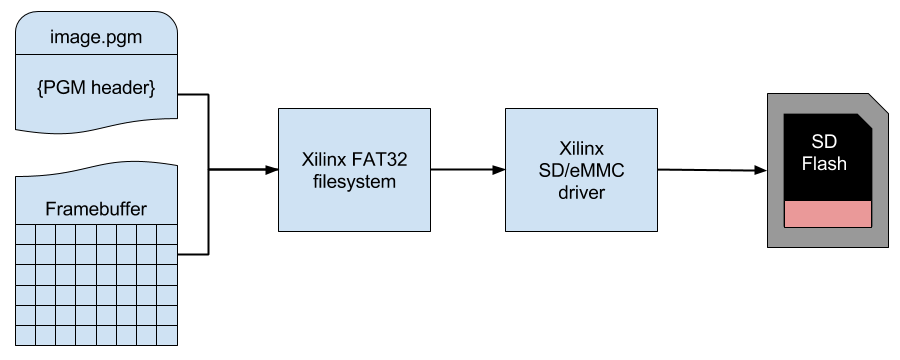
\includegraphics[width=1\textwidth]{./img/flash_storage.png}
  \caption{Framebuffer data is converted into PGM format and written to an SD card using Xilinx's FAT library.}
  \label{fig:flash_storage}
\end{figure}

Due to space constraints the framebuffer is only able to store a single frame at a time; upon receiving a new frame the previous frame is completely overwritten. Even if multiple frame buffers were used, the \SI{512}{\mega\byte} of DDR3 RAM inside the \gls{ps} would be filled after a few seconds of video. Instead, a flash-based SD card is used to store captured images when the shutter release is pressed. 

The Zybo development board used for this proof-of-concept system includes a multitude of built-in peripherals which can be accessed from both the \gls{pl} and the \gls{ps}. A MicroSD slot, SDIO 0, is provided as part of these peripherals and is connected to the \gls{ps} via multiplexed IO bank 1, lines 40--47. SD cards are typically able to run in two modes: SDIO mode (using the SDIO interface for high-throughput) and SPI mode (using the SPI interface for low-throughput). Higher throughput requires more resources and thus SPI mode is typically the preferred choice on resource-constrained microcontrollers. The ARM Cortex A9 inside the Zynq \gls{ps} is a fairly capable microprocessor however, and has full support for the SDIO interface via the SDIO peripheral controller. To read and write to the SD card the controller uses a 4-bit data interface with a maximum clock frequency of \SI{50}{\mega\hertz} for a theoretical transfer rate of \SI{25}{\mega\byte\per\second} --- of course this throughput is highly dependant on the type of data being transferred and the SD card used.

Writing to the SD card involves several layers of abstraction. The first abstraction layer is the Xilinx SD / eMMC library, which abstracts away the registers associated with operation of the SDIO peripheral controller which actually communicates with the SD card. One layer above that is Xilinx's FAT filesystem library which provides a very basic API for working with files stored in a FAT32 filesystem. FAT32 is supported on every major operating system, meaning that the SD card can be mounted and viewed on any system. It is also a relatively simple filesystem, making it the perfect choice for this proof-of-concept project which runs on bare-metal without the convenience provided by a full operating system such as embedded Linux. A Linux kernel for the Zynq platform was compiled from scratch as part of the project, however interfacing with any peripherals in the \gls{pl} would have required writing low-level kernel drivers which is far outside the scope of the project.

\begin{lstlisting}[caption={Using the Xilffs library to write the framebuffer to an SD card.}, label={lst:xilffs}, language=C]
FRESULT status;

// Mount the SD card to 0:/
status = f_mount(&fatfs, root_path, 0);
if (status != FR_OK) {
    return XST_FAILURE;
}

return XST_SUCCESS;

// Open a new PGM file for writing
status = f_open(&fh, filename, FA_CREATE_ALWAYS | FA_WRITE);
if (status != FR_OK) {
    return XST_FAILURE;
}

// Point the file pointer to the start of the file
status = f_lseek(&fh, 0);
if (status != FR_OK) {
    return XST_FAILURE;
}

(void)f_puts("P2\n640 480\n255\n", &fh);

// Flash data cache and write out pixel data
Xil_DCacheFlushRange((UINTPTR)g_framebuf, FRAMEBUF_WIDTH * FRAMEBUF_HEIGHT);
for (line=0; line<FRAMEBUF_HEIGHT; line++) {
    for (pixel=0; pixel<FRAMEBUF_WIDTH; pixel++) {
        f_printf(&fh, "%d ", g_framebuf[line][pixel]);
    }
    f_putc('\n', &fh);
}
\end{lstlisting}

Listing \ref{lst:xilffs} shows the Xilinx FAT filesystem library being used to write a frame to the SD card. Before the SD card can be used it must first be mounted using the \texttt{f\_mount()} function so the filesystem can be accessed --- this is immediately reminiscent of UNIX systems. Once the filesystem is mounted, the Xilffs library provides functions for file access, directory access, file / directory management and volume management (\url{http://www.xilinx.com/support/documentation/sw_manuals/xilinx2014_1/oslib_rm.pdf}). To write a frame to the SD card the \texttt{f\_open()} function is called to open a file, specifying the \texttt{FA\_WRITE} flag to indicate the file is to be written to. Before any data can be written the file pointer must be positioned at the start of the file using the \texttt{f\_lseek()} function with an offset of zero. As with the framebuffer \gls{dma} processor, the data cache needs to be flushed before writing any data otherwise stale data will be used for the \gls{dma} transfer to the SD card. The Xilffs library supports multiple ways of writing to a file; the \texttt{f\_printf()} function is used here to write each pixel in the framebuffer to the file as integers delimited by spaces. It is important to finish any set of writes with a call to \texttt{f\_close()} to ensure that all bytes are committed to the disk.

Due to the transfer rates it is not possible to capture video using this method --- only still images can be captured. When doing anything requiring working with filesystems and high throughput it is generally desirable to use a full operating system with optimised filesystem code. While very lean, programming on bare-metal means not having many of the underlying mechanisms such as IO buffers, which are used to accelerate filesystem access to attain high throughput rates. The Xilinx FAT filesystem library is provided mainly for convenience --- to be able to log small quantities of data to an external SD card, not for pushing out 1080p video.

Because the entire framebuffer is written in one go, the framebuffer \gls{dma} processor is blocked from running. While the \glspl{isr} are still called, the framebuffer \gls{dma} transfers are initiated in the main process which is blocked by the SD card write. As the framebuffer \gls{dma} processor is inactive during this period the output linebuffer becomes stale, with the viewfinder controller rendering the same line repeatedly, causing the pixel smearing in Figure \ref{fig:interrupt_smudge}. While very simple, writing the entire frame in a single chunk is sub-optimal and several markedly better alternatives exist. Firstly, the ARM Cortex A9 inside the \gls{ps} is dual core, however the firmware is only single-threaded. Rather than running everything on a single core, it would be desirable to run critical tasks  (anything involving reading or writing to the framebuffer) on one core and non-critical code (rendering the viewfinder HUD) on the other. Another improvement would be the addition of a state machine; rather than writing the whole chunk in one go, a state machine could be used to break the SD card write into smaller chunks so that the framebuffer \gls{dma} processor can run in between.

\marginpar{insert diagram of this}

\begin{figure}
  \centering
  
\includegraphics[width=1\textwidth]{./img/interrupt_smudge.jpg}
  \caption{Writing to flash storage prevents the framebuffer \gls{dma} processor from running, causing a smudged appearance as the same line is drawn repeatedly.}
  \label{fig:interrupt_smudge}
\end{figure}

\subsection{PGM image format}
Images are saved in \gls{pgm} ASCII format for convenient viewing on computers. \gls{pgm} is very basic greyscale image format designed to be platform-agnostic and thus fully portable between different systems. Typically a RAW format such as Adobe DNG would be used for storing RAW images as they are able to embed additional metadata such as the \gls{cfa} pattern and camera settings (aperture, focal length etc.) used. As a middle-ground between a completely proprietary binary format and standardised but complex RAW format, \gls{pgm} was chosen for its portability and simplicity.

When used in ASCII mode, \gls{pgm} data is encoded as ASCII data using space delimiters, rather than as binary values at specific offsets. The header is simply the magic string \texttt{P2} to identify the ASCII \gls{pgm} file format, followed by the width and height of the image in pixels, followed by \texttt{255}, the maximum value per pixel. The \gls{pgm} header used for the OV7670 image sensor is shown in Listing \ref{lst:pgm_header}.

\begin{lstlisting}[caption={\gls{pgm} file header.}, label={lst:pgm_header}]
P2          # P1 = Bitmap, P2 = Greymap, P3 = Pixmap
640 480     # OV7670 images are 640 x 480
255         # 8-bit pixel-depth
\end{lstlisting}

After the header the pixel data is written out as 480 lines of 640 ASCII-formatted integer values, with each value corresponding to a single pixel. As in the header, values are delimited by spaces. The resulting images are able to be viewed in any \gls{pgm} viewer, or converted to a more common filetype such as a Bitmap or PNG.